s\chapter{Introduction}
\section{Quantum Chromodynamics (QCD)}
\label{sec_1_qcd}
Quantum Chromodynamics (QCD) is a local SU(3) gauge theory and describes the strong interaction of quarks and gluons. 
%Quarks and gluons have color charges and they interact by strong force. 
The Lagrangian of QCD is expressed by, 
\begin{equation}
  L_{QCD} = \bar{\psi_{q}^{i}}( i\gamma^{\mu}(D_{\mu})_{ij} - m_{q}\delta_{ij} ) \psi_{q}^{j} - \frac{1}{4}F_{\mu\nu}^{a}F_{a}^{\mu\nu}
\end{equation}
where $\psi^{i}_q$ is the quark field with color index $i$, $\gamma^{\mu}$ is a Dirac matrix, $m_{q}$ is the quark mass. 
$F^{a}_{\mu\nu}$ is the gluon field strength tensor with gluon color index $a$. 
$(D_{\mu})_{ij}$ is the covariant derivative of QCD expressed by, 
\begin{equation}
  (D_{\mu})_{ij} = \delta_{ij}\partial_{\mu} - ig_{s}t^{a}_{ij}A^{a}_{\mu}
\end{equation}
where $g_{s}$ is the strong coupling constant, and $A^{a}_{\mu}$ is gluon field with gluon color index $a$. 
In QCD, the colored state is prohibited to exist and quarks and gluons are confined in color-singlet hadrons at low energy ("quark confinement''). 
The strong running coupling constant $\alpha_{s}=g_{s}^{2}/4\pi$ can be expressed as a function of the momentum transfer ($Q$), 
\begin{equation}
  \alpha_{s}(Q^{2}) = \frac{12\pi}{(33-2n_{f})ln(Q^{2}/\Lambda^{2}_{QCD})}
\end{equation}
% pQCD is valid
where $n_{f}$ is the number of quark flavors, $\Lambda_{QCD}\sim$ 200 MeV is the typical QCD scale. 
If $Q^{2} >> \Lambda_{QCD}^{2}$ (short-range interaction), the $\alpha_{s}$ becomes small. 
This feature is called as "asymptotic freedom''. 
Figure~\ref{fig_1_alphas} shows the $\alpha_{s}$ measurements as a function of Q~\cite{bib_pdg}.
\begin{figure}[!h]
  \centering
  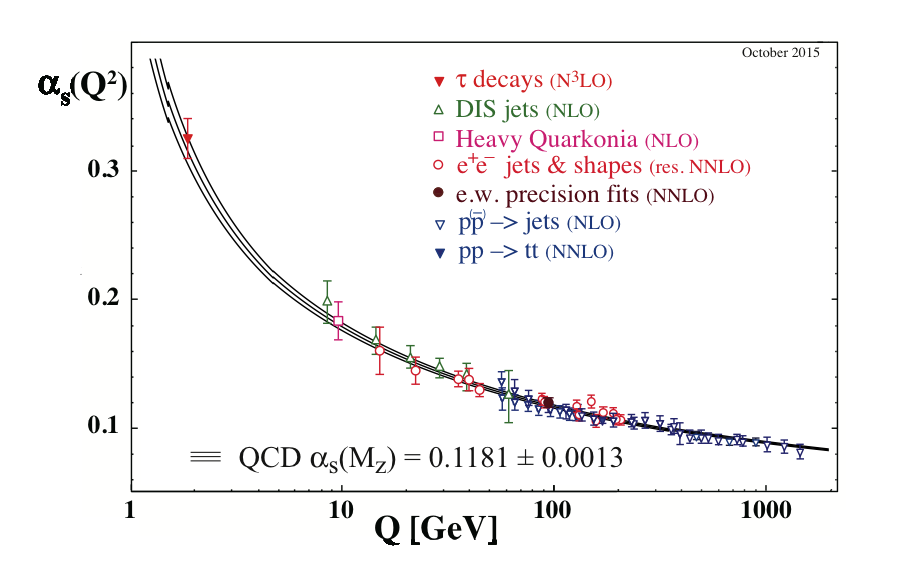
\includegraphics[width=10cm]{chap1/figure/alphas.eps}
  \caption{Summary of measurements of $\alpha_{s}$ as a function of the Q. The respective degree of QCD perturbation theory used in the extraction of $\alpha_{s}$ is indicated in brackets (NLO: next-to-leading order, NNLO: next-to-next-to leading order,  NNLO: NNLO matched with resumed next-to-leading logs, $\rm{N^{3}LO}$:next-to-NNLO)~\cite{bib_pdg}.}
  \label{fig_1_alphas}
\end{figure}

\section{Quark Gluon Plasma (QGP)}
Due to the asymptotic freedom, the coupling of QCD is estimated to become weak at high temperature. %~\cite{bib_alphatemp}.
Therefore it is anticipated that the confinement may be broken in high temperature or high density matters and the phase transition to a deconfined state called quark-gluon plasma (QGP) occurs. 
It is thought that the phase transition to QGP in heavy ion collisions at the Large Hadron Collider (LHC) described in the next section is not a first order phase transition but a crossover where there is not a clear separation of phases but the thermodynamic properties change rapidly around the critical temperature $T_{c}$. 
Figure~\ref{fig_1_lattice} shows the results of the (2+1) lattice calculation on the pressure (3p/$T^{4}$), energy density($\epsilon/T^{4}$), and entropy density ($3s/4T^{3}$) as a function of temperature when the chemical potential $\mu$ is zero\cite{bib_hotqcdlattice}.
According to this calculation, $T_{c}$ is expected 154 $\pm$ 9 MeV. 
Below $T_{c}$, the calculated results with the lattice QCD shows the reasonable agreement to the  hadron resonance gas model (HRG) which assumes all hadrons or hadron resonance states contribute to the thermodynamics as non-interacting particles.
Above $T_{c}$, the estimations of HRG lie along the lower edge of the lattice predictions and show the discrepancies from the lattice calculation as the temperature rises. 
%The results of the lattice calculation doesn't show the flat shape but an asymptotic growth to the Stefan-Boltzmann limit at high temperature. 
The results of the lattice calculation doesn't show the flat shape and underestimates compared to the Stefan-Boltzmann limit. 
It implies the interaction of gluons and quarks in the QGP might not be so weak coupled as to be approximated by the ideal gas.
\begin{figure}[!h]
	 \centering
	 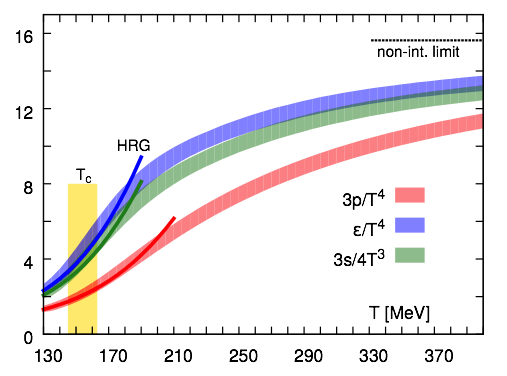
\includegraphics[width=10cm]{chap1/figure/hotqcdlattice.png}
  	\caption{ Calculated result of lattice QCD on the energy density, entropy density, and pressure as a function of temperature $T$~\cite{bib_hotqcdlattice}.}
 	 \label{fig_1_lattice}
\end{figure}

%The lattice calculation predict the critical temperature ($T_{c}$) of the phase transition to QGP is 150-200 MeV. 
%Figure~\ref{fig_1_lattice} shows the calculated result of the entropy density $s/T^{3}$ as a function of temperature $T$~\cite{bib_slattice}.  
%The entropy increases close to the Steffen-Boltzmann limit rapidly around 200 MeV due to the increase of the degree of freedom.
%The increase of degree of freedom is attributed by the creation of deconfiend state composed of quarks and gluons. 
%Figure~\ref{fig_1_lattice} shows the results of the (2+1) lattice calculation on the pressure (3p/$T^{4}$), energy density($\epsilon/T^{4}$), and entropy density ($3s/4T^{3}$) as a function of temperature.
%This model take into account two light quark flavor with the same mass and one heavy flavor tuned to match the $\eta_{s\bar{s}}$ mass. 
%In the ideal gas limit, the system obeys Steffen-Boltzmann low and these values become constant. 
%The yellow band in Fig.~\ref{fig_1_lattice} shows the crossover region around the critical temperature 145 $<$ $T$ $<$ 164 MeV.
%Below 150 MeV, the results show the agreement to the hadron resonance gas approximation. 
%The discrepancy between two approximation is shown above 170 MeV. 
%They are not saturated at higher temperature but the energy density and the entropy density increase rapidly around $T_{c}$ due to the increase of the degree of freedom by the transition from the hadronic matter to the partonic matter.
%\begin{figure}[!h]
 % \centering
%  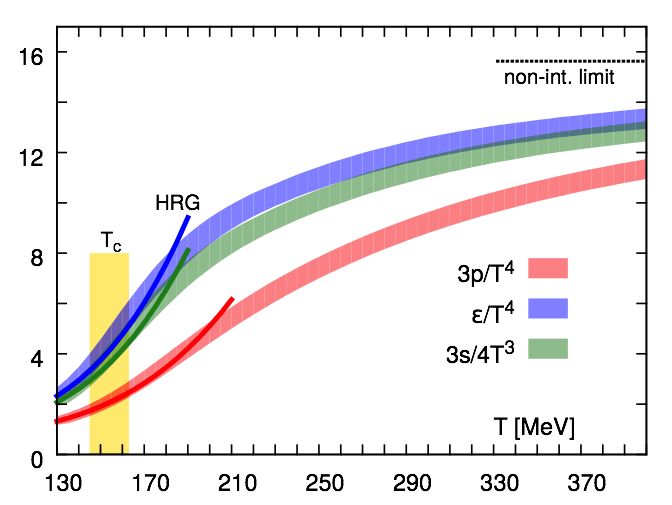
\includegraphics[width=8cm]{chap1/figure/lattice.png}
%  \includegraphics[width=10cm]{chap1/figure/latticeentropy.png}
%  \caption{ Calculated result of lattice QCD on the entropy density ($s/T^{3}$) as a function of temperature $T$~\cite{bib_slattice}.}
%  \label{fig_1_lattice}
%\end{figure}
%The lattice calculation of QCD predicts that the phase transition occurs around the critical temperature $T_{c}\sim$ 150-200 MeV. 
%Figure~\ref{} shows the calculated result of the entropy density as a function of temperature. 
%The entropy density increases  at $T\sim$ 200 MeV due to the increase of the degree of freedom, which imply the existence of the de-confined state. 


\section{Relativistic Energy Heavy Ion Collisions}
Relativistic heavy ion collisions are thought as the unique tool to create the QGP in the laboratory.
For example, the initial energy density of Pb-Pb collisions at LHC calculated by the Bjorken formula is $\epsilon_{0}\sim$ 20 GeV/$\rm{fm}^{3}$. 
%$A$ is the transverse are and $c\tau_{0}$ is longitudinal length of the considered initial 
%$\tau_{0}$ is assumed 0.08 fm.
It is much higher than the expected QGP threshold $\epsilon_{c}$ ($\sim$ 1 GeV/$\rm{fm}^{3}$).
The temperature is expected to reach up to 4 $T_{c}$.
Therefore it is believed that QGP is created in relativistic heavy ion collisions. 

The first experiment of the relativistic heavy ion collisions is performed at Bevalac in Lawrence Berkeley in the middle of 1970’s.
It is a Fixed-target experiment with the energy per nucleon of 2 A GeV.  
In 1980's, the experiments at the Alternating Gradient Synchrotron (AGS) in Brookhaven National Laboratory (BNL) and Super Proton Synchrotron (SPS) in European Organization for Nuclear Research (CERN) started with the beam energy per nucleon of $\sim$ 14A GeV and $\sim$ 160A GeV, respectively. 
The Relativistic Heavy Ion Collider (RHIC) in BNL is the first collider for the relativistic heavy ion collisions. 
The Large Hadron Collider (LHC) in CERN provides heavy ion collisions since 2010.  

Figure~\ref{fig_1_hic} shows the schematic view of the space-time evolution of heavy ion collisions~\cite{bib_spacetime}. 
It is necessary to understand the space-time evolution of heavy-ion collisions to study the formation of the QGP.
\begin{figure}[!h]
  \centering
  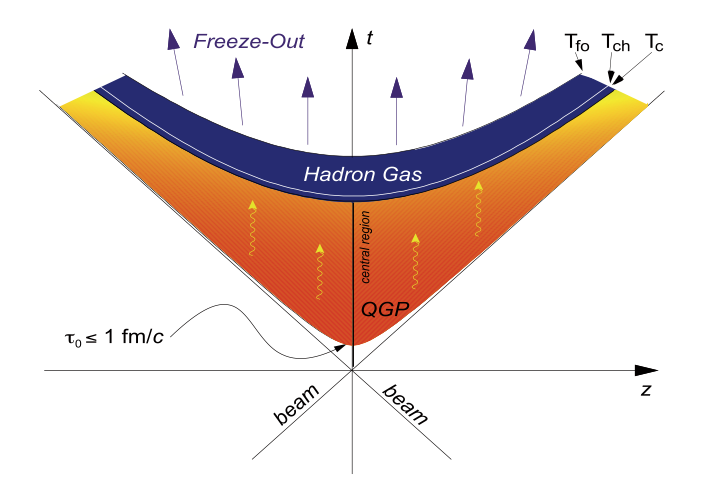
\includegraphics[width=12cm]{chap1/figure/hic.png}
  \caption{Space and Time evolution in relativistic heavy ion collisions. The z-axis express the beam direction. $\tau_{0}$ is the formation time of QGP. $T_{c}$, $T_{ch}$ ,and $T_{fo}$ denote critical temperature, chemical freezeout temperature, and kinematical freezeout temperature, respectively~\cite{bib_spacetime}.}
  \label{fig_1_hic}
\end{figure}
The space-time evolution of heavy ion collisions can be separated into the initial stage before collisions, pre-equilibrium stage, equilibrium stage (QGP) and expansion of the QGP, hadronic gas phase, chemical freezeout, and kinematical freezeout.
It is assumed that the space-time evolution is dependent on only the proper time $\tau=\sqrt{t^{2}-z^{2}}$ at high energy limit. 
\begin{description}
\item[Initial Stage] \mbox{}\\
When the nuclei collide at $\tau=$0, a large number of nucleon-nucleon collisions occur in the overlap region of incident nuclei. % and huge amount of energy is deposited in a small volume. 
It is non-trivial that heavy-ion collisions can be described by the superposition of nucleon-nucleon collisions due to the existence of normal nuclear effects as described in Chapter 2.
%This initial nucleus-nucleus collisions cannot is not exactly same as the superposition of the nucleon-nucleon collisions because of nuclear matter effects described in Chapter~\ref{chap_phys}.
The system is not thermalized at this points.

\item[Pre-equilibrium stage] \mbox{} \\
After initial collisions, a large amount of color flux tubes are generated between passing nuclei along the beam axis. 
This state is called as "Glasma".
Due to their instabilities, they decay into partons and the system reaches the local equilibrium at the formation time $\tau = \tau_{0}$. 
If the temperature is above the $T_{c}$ at $\tau=\tau_{0}$, QGP is formed. 
%%$\tau_{0}$ is expected very short within 1 fm/$c$.
The exact $\tau_{0}$ value is still unknown but it is estimated to be at least shorter than 1 fm/$c$~\cite{bib_flow}.


\item[Equilibrium stage (QGP) and expansion of the QGP] \mbox{} \\
Once the system becomes thermalized, the expansion of the system can be described by the relativistic hydrodynamics. 
%During the collective expansion of the system, the temperature drops and if it crosses the $T_{c}$, hadrons are generated 
The system cools down and if the temperature is below $T_{c}$, the hadrons start to be created and the system is dominated by hadrons. 

\item[Hadron gas phase] \mbox{} \\
As temperature of hadron gas decrease and when the temperature cross the chemical freezeout temperature $T_{ch}$, the relative particle ratio of hadrons are fixed although generated hadrons interact each other. 
At the kinetic freezeout temperature $T_{fo}$, the momentum distribution of hadrons is fixed and hadrons are emitted from the matter.  
\end{description}
%RHIC and LHC provides many signs of the QGP formation such as $J/\psi$ suppression and large anisotropic flow\cite{bib_jpsiaarhic}. 
%However, in order to extract QGP signal from the experimental data, whole understanding of the space-time evolution of the heavy ion collision is needed. 
The comparison between the experimental results and hydrodynamic calculation indicates that the system expands collectively with small shear viscosity to entropy density ratio ($\eta /s$) close to the lower bound 1/4$\pi$~\cite{bib_flow}. 
It implies that partons in the QGP interact strongly and the mean free path is sufficiently short compared to the system size. 


\section{Objective and Organization of Thesis}
$J/\psi$ has been considered as one of the golden probes to discuss the formation of the QGP.
As is described in Chapter 2, attraction between $c$ and $\bar{c}$ quarks is reduced by Color Debye screening in QGP and thus $J/\psi$ is not formed in the QGP.
In addition to the color screening effect in the QGP, normal nuclear matter effects such as the gluon shadowing play a role to modify the $J/\psi$ production in heavy-ion collisions. 
Understanding of the normal nuclear matter effects is mandatory for the understanding of the QGP effects to the $J/\psi$ production in heavy-ion collisions.
In this thesis, $J/\psi$ production in p-Pb collisions at the LHC is measured and normal nuclear effects to the $J/\psi$ production is described.

The organization of this thesis is as follows.  
In Chapter~\ref{chap_phys}, the physics background related to this thesis is summarized. 
In Chapter~\ref{chap_setup}, the LHC complex and the detector setup of the ALICE experiment is described. 
In Chapter~\ref{chap_ana}, the analysis of $J/\psi\rightarrow e^{+}e^{-}$ in p-Pb collisions at $\sqrt{s_{NN}}=$5.02 TeV is explained. 
In Chapter~\ref{chap_dis}, experimental results and their interpretation are discussed. 
The conclusion of this thesis is summarized in Chapter~\ref{chap_con}

\section{Major Contribution}
As one of the members in ALICE collaboration, the author carried out data taking of the ALICE experiment. 
In addition, the major contributions of the author are following. 
\begin{description}
  \item{-} Installation, commissioning, and operation of the Transition Radiation Detector (TRD).
  %\item{-} The feasibility and conceptual design study of the new scheme of the TRD pretrigger. 
  \item{-} Study of the trigger efficiency of the electron triggers with TRD in p-Pb collisions.
  \item{-} Dielectron analysis in p-Pb collisions described in this thesis.
\end{description}



